\documentclass[14pt,a4paper,oneside]{report}		%lớp văn bản
\usepackage{graphicx}
\graphicspath{{images/}}
\usepackage[utf8]{vietnam}						%gói ngôn ngữ tiếng Việt
%--
\usepackage{fancybox}
\usepackage{amsfonts}
\usepackage{latexsym, amsmath, amsxtra, amssymb, amscd, amsthm}	%gói ký tự toán
\usepackage{indentfirst}
\usepackage{fancyheadings}
\usepackage{color,colortbl}		%gói màu
\usepackage{graphicx}			%gói hình ảnh 
\usepackage{hyperref}			%gói liên kết link
\usepackage[top=3.5cm, bottom=3.0cm, left=3.5cm, right=2cm] {geometry}
\lhead{Mô hình ngẫu nhiên và ứng dụng}
\rhead{Nhóm 2 - Toán Tin K58}
%//================================= Begin dinh nghia cac goi lenh
\renewcommand{\contentsname}{Mục lục}
\renewcommand{\chaptername}{Chương}
\renewcommand\bibname{Tài liệu tham khảo}
\newcommand{\gach}{\backslash}
\newtheorem{theorem}{Định lý}
%==================================// End dinh nghia cac goi lenh
%//================================== Begin make title
\title{{\bf  BÁO CÁO CUỐI KỲ MÔN MÔ HÌNH NGẪU NHIÊN VÀ ỨNG DỤNG}}
\author{Phạm Thanh Sơn, Nguyễn Lê Hoàng\\Phạm Hữu Nghị, Vũ Hải Trường}

\date{{\em \today}}
%==================================// End make  title
\begin{document}

\thispagestyle{empty}
\thisfancypage{
\setlength{\fboxsep}{0pt}
\fbox}{} 
\begin{center}
\begin{large}
TRƯỜNG ĐẠI HỌC BÁCH KHOA HÀ NỘI
\end{large} \\
\begin{large}
VIỆN TOÁN ỨNG DỤNG VÀ TIN HỌC
\end{large} \\
\textbf{--------------------  *  ---------------------}\\[2.5cm]
\includegraphics[width=3cm,height=3cm,keepaspectratio]{logo.jpg}\\[2.5cm]
{\fontsize{32pt}{1}\selectfont BÁO CÁO MÔN HỌC}\\
{\fontsize{20pt}{1}\selectfont CÁC MÔ HÌNH NGẪU NHIÊN VÀO ỨNG DỤNG}\\[2cm]
{\fontsize{15pt}{1}\selectfont Đề tài: Học tăng cường}\\[1cm]
\end{center}

\hspace{5cm} Mhóm sinh viên thực hiện : \hspace{4pt}
\textbf{\parbox[t]{5cm}{    
Phạm Thanh Sơn\\
Nguyễn Lê Hoàng\\
Phạm Hữu Nghị\\
Vũ Hải Trường
}}\\[12pt]

\hspace{5cm} Giáo viên hướng dẫn \hspace{24pt} :  \hspace{4pt} \textbf{\parbox[t]{5cm}{    
Ts. Nguyễn Thị Ngọc Anh
}}

\vspace{3cm}
\begin{center}
{\fontsize{16pt}{1}\selectfont HÀ NỘI}\\
{\fontsize{16pt}{1}\selectfont \today}
\end{center}

\pagestyle{fancy}	
\Large												%co chu
\maketitle											%make title
\setlength{\baselineskip}{5truept}		%gian dong cho muc luc
\tableofcontents									%tao muc luc
\newpage
\setlength{\baselineskip}{18truept}	%gian dong cho van ban
%//==========================================Begin noi dung bai==
\chapter{Giới thiệu}
Trong ngành khoa học máy tính, học tăng cường (tiếng Anh: reinforcement learning) là một lĩnh vực con của học máy, nghiên cứu cách thức một tác tử (agent) trong một môi trường nên chọn thực hiện các hành động nào để cực đại hóa một khoản thưởng (reward) nào đó về lâu dài. Các thuật toán học tăng cường cố gắng tìm một chiến lược ánh xạ các trạng thái của thế giới tới các hành động mà agent nên chọn trong các trạng thái đó.

Môi trường thường được biểu diễn dưới dạng một quá trình quyết định Markov trạng thái hữu hạn (Markov decision process - MDP), và các thuật toán học tăng cường cho ngữ cảnh này có liên quan nhiều đến các kỹ thuật quy hoạch động. Các xác suất chuyển trạng thái và các xác suất thu lợi trong MDP thường là ngẫu nhiên nhưng lại tĩnh trong quá trình của bài toán (stationary over the course of the problem).

Khác với học có giám sát, trong học tăng cường không có các cặp dữ liệu vào/kết quả đúng, các hành động gần tối ưu cũng không được đánh giá đúng sai một cách tường minh. Hơn nữa, ở đây hoạt động trực tuyến (on-line performance) được quan tâm, trong đó có việc tìm kiếm một sụ cân bằng giữa khám phá (lãnh thổ chưa lập bản đồ) và khai thác (tri thức hiện có). Trong học tăng cường, sự được và mất giữa khám phá và khai thác đã được nghiên cứu chủ yếu qua bài toán multi-armed bandit.
%==============================
\chapter{Phương pháp}
Chương đầu có nội dung như sau

\section{Quá trình quyết định Markov}
Quá trình quyết định Markov (MDP) cung cấp một nền tảng toán học cho việc mô hình hóa việc ra quyết định trong các tình huống mà kết quả là một phần ngẫu nhiên và một phần dưới sự điều khiển của một người ra quyết định. MDP rất hữu dụng cho việc học một loạt bài toán tối ưu hóa được giải quyết thông qua quy hoạch động và học tăng cường. MDP được biết đến sớm nhất là vào những năm 1950 (cf. Bellman 1957). Một cốt lõi của nghiên cứu về quá trình ra quyết định Markov là từ kết quả của cuốn sách của Ronald A. Howard xuất bản năm 1960, Quy hoạch động và quá trình Markov. Chúng được sử dụng trong rất nhiều các lĩnh vực khác nhau, bao gồm robot, điều khiển tự động,kinh tế, và chế tạo.

Chính xác hơn, một quá trình quyết định Markov là một quá trình điều khiển ngẫu nhiên thời gian rời rạc. Tại mỗi bước thời gian, quá trình này trong một vài trạng thái $s$, và người ra quyết định có thể chọn bất kỳ hành động $a$ nào có hiệu lực trong trạng thái $s$. Quá trình này đáp ứng tại bước thời gian tiếp theo bằng cách di chuyển ngẫu nhiên vào một trạng thái mới $s'$, và đưa ra cho người ra quyết định một phần thưởng tương ứng $R_a(s,s')$.

Xác suất mà quá trình di chuyển vào trạng thái mới của nó $s'$ bị ảnh hưởng bởi hành động được chọn. Đặc biệt, nó được đưa ra bởi hàm chuyển tiếp trạng thái $P_a(s,s')$. Do đó, trạng thái kế tiếp $s'$ phụ thuộc vào trạng thái hiện tại s và hành động của người ra quyết định $a$. Nhưng $s$ và $a$ đã cho, lại độc lập có điều kiện với toàn bộ trạng thái và hành động trước đó; nói cách khác, các trạng thái chuyển tiếp của một quá trình MDP thỏa mãn thuộc tính Markov.

Quá trình quyết định Markov là một phần mở rộng của chuỗi Markov; khác biệt là ở sự bổ sung của các hành động (cho phép lựa chọn) và phần thưởng (cho động cơ). Ngược lại, nếu chỉ có một hành động tồn tại cho mỗi trạng thái và tất cả các phần thưởng là giống nhau (ví dụ: zero), một quá trình quyết định Markov làm giảm một chuỗi Markov.
\subsection{Quá trình quyết định Markov}
Để dễ dàng triển khai, chúng ta chỉ quan tâm đến các quá trình Markov đếm được và hệ số chiết khấu tiêu chuẩn. Tuy nhiên, trong một số điều kiện kỹ thuật, kết quả cũng được mở rộng ra cho các quá trình quyết định Markov liên tục liên tục.\\
Một quá trình quyết định Markov $\mathcal{M} = (\mathcal{X},\mathcal{A},\mathcal{P}_0)$, với $\mathcal{X}$ là tập các trạng thái đếm được khác rỗng, $\mathcal{A}$ tập các hành động ($\mathcal{A}$ cũng là tập đếm được và khác rỗng). $\mathcal{P}_0$ là tập các xác suất chuyển ứng với mỗi cặp trạng thái và hành động tương ứng $(x,a) \in \mathcal{X}\times\mathcal{A}$ một độ đo xác suất trên $\mathcal{X}\times\mathbb{R}$ mà chúng ta định nghĩa bởi $\mathcal{P}_0(.|x,a)$. $\mathcal{P}_0$ có thể hiểu: cho $\mathcal{U}\subset\mathcal{X}\times\mathbb{R}$, $\mathcal{P}_0(U|x,a)$ là xác suất mà trạng thái kế tiếp và phần thưởng của $\mathcal{U}$ với trạng thái hiện tại là $x$, và hành động được thực hiện là $a$. Hệ số chiết khấu $\gamma$ với $0\leq \gamma\leq 1$.\\
Xác suất chuyển trạng thái $\mathcal{P}$ với mỗi $(x,a,y)\in\mathcal{X}\times\mathcal{A}\times\mathcal{X}$ sẽ được cho bởi xác suất chuyển từ trạng thái $x$ đến một trạng thái $y$ nào đó mà hành động $a$ được thực hiện từ trạng thái $x$:
$$\mathcal{P}(x,a,y)=\mathcal{P}_0(\{y\}\times|x,a).$$
Ngoài $\mathcal{P}$, $\mathcal{P}_0$ cũng làm tăng hàm phần thưởng $r:\mathcal{X}\times\mathcal{A}\rightarrow\mathbb{R}$, là phần thưởng khi ta ở trạng thái $x$ thực hiện hành động $a$: nếu $(Y_{(x,a)},R_{x,a})\sim\mathcal{P}_0(.|x,a)$ thì:
$$r(x,a)=\mathbb{E}[R_{(x,a)}].$$
Chúng ta giả sử các phần thưởng bị chặn bởi $\mathcal{R} > 0$: với mọi cặp $(x,a) \in \mathcal{X}\times\mathcal{A}, |R_{(x,a)}|\leq\mathcal{R}$. Nếu hàm phần thưởng bị chặn bởi $\mathcal{R}$ thì $||r||_\infty = \text{sup}_{(x,a)\in\mathcal{X}\times\mathcal{A}}|r(x,a)|\leq\mathcal{R}$. Một quá trình quyết định Markov được gọi là hữu hạn nếu cả hai tập $\mathcal{X}$ và $\mathcal{A}$ là hữu hạn.\\
Quá trình quyết định Markov là một công cụ để mô hình hóa các vấn đề ra quyết định khi người ra quyết định tương tác với hệ thống theo một cách tuần tự. Cho quá trình quyết định Markov $\mathcal{M}$ như sau: cho $t\in\mathbb{N}$ là thời điểm hiện tại (hoặc trạng thái hiện tại), gọi $X_t\in\mathcal{X}$ và $A_t\in\mathcal{A}$ là một trạng thái trong hệ thống và hành động được chọn tại thời điểm $t$. Mỗi hành động được chọn là một quá trình biến đổi:
$$(X_{t+1},R_{t+1})\sim\mathcal{P}_0(\cdotp|X_t,A_t).$$
Đặc biệt, $X_{t+1}$ là ngẫu nhiên và $\mathbb{P}(X_{t+1}=y|X_t=x,A_t=a)=\mathcal{P}(x,a,y)$ với mọi $x,y\in\mathcal{X}, a\in\mathcal{A}$. Hơn nữa, $\mathbb{E}[R_{t+1}|X_t,A_t]=r(X_t,A_t)$. Người đưa ra quyết định sẽ xem trạng thái tiếp theo $\mathcal{X}_{t+1}$ và phần thưởng $R_{t+1}$ để chọn hành động $A_{t+1}\in\mathcal{A}$ và quá trình đó được lặp đi lặp lại. Mục tiêu là tìm ra cách để lựa chọn hành động sao cho cực đại tổng khoản thưởng chiết khấu.\\

Người đưa ra quyết định có thể chọn hành động ở bất cứ trạng thái nào dựa trên lịch sử quan sát. Cứ mỗi hành động được chọn được gọi là một hành vi. Hành vi quyết định và tập các trạng thái bắt đầu $X_0$ là một trạng thái hành động phần thưởng ngẫu nhiên $((X_t,A_t,R_{t+1});t\geq 0)$, $A_t$ là hành động được quy định bởi các hành vi dựa trên lịch sử $X_0,A_0,R_1,...,X_{t-1},A_{t-1},R_t,X_t.$. Lợi nhuận của một hành vi được định nghĩa dựa trên tổng chiết khấu của phần thưởng:
$$\mathcal{R}=\displaystyle\sum_{t=0}^{\infty}{\gamma^tR_{t+1}}.$$
Nếu $\gamma < 1$ thì phần thưởng ở tương lai sẽ nhỏ hơn phần thưởng ở trạng thái ban đầu. Một quá trình quyết định Markov khi mà lợi nhuận được định nghĩa theo công thức thì được gọi là chiết khấu phần thưởng MDP. Khi $\gamma =1$ thì quá trình quyết định Markov được gọi là không chiết khấu.\\
Mục tiêu của người ra quyết định lựa chọn hành vi để cực đại kỳ vọng lợi nhuận, khi nào quá trình bắt đầu.\\
Ví dụ 1 (Kiểm soát hàng tồn kho): Xét một vấn đề hàng ngày về kiểm soát hàng tồn kho: mỗi tối, quản lý phải đưa ra quyết định về số lượng hàng được đặt trong ngày hôm sau. Sáng hôm sau, lượng hàng đã được đặt sẽ chuyển vào kho. Trong ngày, một số nhu cầu ngẫu nhiên được thực hiện, nhu cầu này là độc lập. Mục tiêu là cực đại giá trị kỳ vọng lợi nhuận trong tương lai. \\
Các khoản phải trả tại thời điểm $t$ được xác định: Chi phí mua hàng $A_t$ là $K\mathbb{I}_{\{A_t>0\}} + cA_t$. Có một chi phí cố định $K$ khác không và mỗi mặt hàng được đặt có giá cố định $c$. $K, c > 0$. Ngoài ra, chi phí duy trì kho của kích thước $x > 0$. Ở trường hợp đơn giản nhất, chi phí này tỷ lệ thuận với kích thước của kho với hệ số $h>0$. Cuối cùng, khi bán được $z$ đơn vị sản phẩm thì thu được $pz$, $p>h>0$.\\
Vấn đề này có thể biểu diễn thành một quá trình quyết định Markov: Gọi $X_t$ là trạng thái tại ngày $t\geq 0$ là kích thước của kho tối hôm đó. $\mathcal{X}=\{0,1,...,M\}$ với $M\in\mathbb{N}$ là kích thước tối đa của kho. Hành động $A_T$ số hàng được đặt tại tối hôm $t$. $\mathcal{A} = \{0,1,...,M\}$ vì số lượng hàng được đặt không vượt quá kích thước của kho. Cho $X_t$ và $A_t$, khoảng trống của kho trong ngày hôm sau là:
\begin{equation} \label{eq2}
X_{t+1}=((X_t+A_t)\wedge M-D_{t+1})^+,
\end{equation}
trong đó $a\wedge b$ là số nhỏ nhất trong hai số $a, b, (a)^+=a\vee 0 =$max$(a,0)$ và $D_{t+1} \in \mathbb{N}$ là nhu cầu của ngày thứ $t+1$. Theo giả thiết, $(D_t;t>0)$ là một dãy phân phối độc lập và đươc phân loại các biến ngẫu nhiên có giá trị nguyên. Doanh thu ở ngày $t+1$ là :
\begin{equation} \label{eq3}
\begin{split}
R_{t+1} = & -K\mathbb{I}_{\{A_t>0\}}-c((X_t+A_t)\wedge M-X_t)^+ \\
& -hX_t + p((X_t+A_t)\wedge M-X_{t+1})^+.
\end{split}
\end{equation}
Công thức \ref{eq2} - \ref{eq3} có thể viết lại dưới dạng:
\begin{equation} \label{eq4}
(X_{t+1},R_{t+1})=f(X_t,A_t,D_{t+1}),
\end{equation}

với một hàm lựa chọn $f$. Khi đó $\mathcal{P}_0$ được xác định:
$$\mathcal{P}_0(U|x,a)=\mathbb{P}(f(x,a,D)\in U) = \displaystyle\sum^\infty_{d=0}{\mathbb{I}_{\{f(x,a,d)\in U\}p_D(d)}}.$$

$p_D(d)$ là xác suất hàm khối lượng ngẫu nhiên yêu cầu và $D\sim p_D(d)$. Điều này hoàn thành định nghĩa của quá trình quyết định Markov trong bài toán tối ưu về hàng tồn kho. \\

Kiểm soát hàng tồn kho chỉ là một trong nhiều vấn đề nghiên cứu dẫn đến quá trình quyết định Markov. Các vấn đề khác bao gồm tối ưu hệ thống giao thông vận tải, sắp xếp lịch hay sản xuất. MDPs phát sinh tự nhiên trong nhiều vẫn đề về kỹ thuật như kiểm soát tối ưu các hệ thông hóa học, điện tử, cơ khí. Khá nhiều vấn đề lý thuyết thông tin có thể cũng được trình bày dưới dạng MDP (ví dụ: mã hóa tối ưu, tối ưu hóa phân bổ kênh hoặc cảm biến mạng). Một vấn đề quan trọng khác là vấn đề tài chính.Bao gồm, quản lý danh mục đầu tư tối ưu và giá cả tùy chọn.\\
Trong trường hợp kiểm soát hàng tồn kho, MDP đã được xác định một cách thuận tiện bởi một hàm chuyển tiếp f (cf., \ref{eq4}). Trong thực tế, các chức năng chuyển tiếp cũng mạnh mẽ như lõi chuyển: bất kỳ MDP nào tạo ra một số chức năng chuyển tiếp f và bất kỳ chức năng chuyển tiếp nào làm tăng MDP.\\
Trong một số vấn đề, không phải tất cả các hành động đều có ý nghĩa ở tất cả các trạng thái. Ví dụ: đặt hàng nhiều mặt hàng hơn so với những gì có chỗ trong kiểm kê không có ý nghĩa nhiều. Tuy nhiên, các hành động vô nghĩa (hoặc các hành động bị cấm) luôn có thể được sửa lại thành hành động khác, giống như nó đã được thực hiện ở trên. Trong một số trường hợp, điều này là bất thường. Sau đó, có thể tốt hơn, ta bổ sung các hành động được chấp nhận cho mỗi trạng thái.
Trong vài trường hợp, một số trạng thái không thể chuyển sang trạng thái khác được hay còn được gọi là trạng thái hấp thụ. MDP có trạng thái hấp thụ thì thường xét phần thưởng không chiết khấu hay $\gamma =1$\\

Ví dụ 2: Một người chơi một trò chơi, tỷ lệ đặt cược $A_t \in [0,1]$ trên tổng số vốn $X_t \geq 0$. Nếu thắng sẽ nhận lại tiền cọc với xác suất $p\in [0,1]$, nếu thua thì sẽ mất tiền cọc với xác suất là $1-p$. Tài sản của người đó được tính:
$$X_{t+1}=(1+S_{t+1}A_t)X_t.$$
$(S_t;t\geq 1)$ là một biến ngẫu nhiên độc lập nhận giá trị $\{-1,+1\}$ với $\mathbb{P}(S_{t+1}=1)=p$. Mục tiêu là cực đại xác suất mà tài sản của người đó đạt giá trị $w^* >0$. Giả sử, ban đầu số tài sản nằm trong khoảng $[0,w^*]$. Bài toán này có thể cọi là một quá trình quyết định Markov với không gian các trạng thái $\mathcal{X}=[0,w^*]$ và tập các hành động $\mathcal{A}=[0,1].$ Ta định nghĩa:
\begin{equation} \label{eq5}
X_{t+1}=(1+S_{t+1}A_t)X_t\wedge w^*,
\end{equation}
trong đó $0\leq X_t \leq w^*$ và $w^*$ là trạng thái kết thúc: $X_{t_1}=X_t$ nếu $X_t=w^*$. Phần thưởng bằng 0 nếu $X_{t+1} < w^*$ và bằng 1 nếu là lần đầu tiên đạt trạng thái $w^*$:
$$R_{t+1} = \begin{cases} 1, & X_t < w^* \mbox{ và } X_{t+1} = w^* \\ 
0, & \mbox{ còn lại } \end{cases}$$
\subsection{Hàm giá trị}
Một các dễ thấy để tìm hành vi tối ưu trong một số quá trình quyết định Markov là liệt kê tất cả các hành vi và chỉ ra hành vi cho giá trị cao nhất với môĩ trạng thái ban đầu. Trên thực tế, các hành vi thuường rất nhiều , và phương pháp này tỏ ra không khả thi. Một các tiếp cận tốt hơn là dựa trên tính toán các hàm giá trị. Trong cách tiếp cận này, người ta tính toán cái gọi là hàm giá trị tối ưu, để rồi sau đó xác định một hành vi tối ưu nhất một cách dễ dàng.
Gái trị tối ưu $V*(x)$, của trạng thái $x \in X$ cho giá trị kỳ vọng cao nhất có thể đạt được khi quá trình bắt đầu từ trạng thái $x$. Hàm $V* : X \rightarrow \mathbb{R}$ được gọi là hàm giá trị tối ưu. Một hành vi được gọi là tối ưu nếu nó đạt  những giá trị tối ưu trong tất cả các trạng thái.\\
Chiến lược dừng tất định (Deterministic stationary policies) thể hiện tập các hành vi đặc biệt, đóng một vai trò quan trọng trong lý thuyết MDP. Chúng được chỉ định bởi một số ánh xạ $\pi$ ($\pi : \mathcal{X}\rightarrow\mathcal{A}$). Tuân theo chiến lược $\pi$ tức là tại mọi thời điểm $t \geq 0$ thì hành động $A_t$ được chọn bằng cách:
\begin{equation} \label{eq6}
A_t = \pi (X_t)
\end{equation}
Thông thuường, một chiến lược ngẫu nhiên dừng (stochastic stationary policy) $\pi$ ánh xạ các trạng thái để phân phối không gian các hành động. Khi đề cập đến 1 chiến lược $\pi$, chúng ta kí hiệu $\pi (a|x)$ để biểu diễn xác suất để hành động $a$ được chọn bởi $\pi$ ở trạng thái $x$. Chú ý rằng nếu một chiến lược trong quá trình quyết định Markov thỏa mãn 
$$A_t  \sim \pi (\cdotp | X_t),  t \in \mathbb{N},$$ thì quá trình trạng thái $(X_t; t \geq 0)$ là một xích Markov. Chúng ta sử dụng $\Pi_stat$ để ký hiệu cho tập tất cả các chiến lược dừng.  Một chiến lược và 1 quá trinh quyết định Markov thì được gọi là Quá trình Markov có phần thưởng (Markov reward processes): Một MRP được xác định bởi cặp $\mathcal{M} = (\mathcal{X},\mathcal{P}_0)$, trong đó $\mathcal{P}_0$ là một xác suất tính dựa vào $\mathcal{X} x \mathbb{R}$ với mỗi trạng thái. Một MRP $\mathcal{M}$ làm tăm quá trình ngẫu nhiên $((X_t,R_{t+1});t\geq 0)$, tại $(X_{t+1},R_{t+1}) \sim \mathcal(P)_0(\cdotp | X_t)$. Cho một chiến lược dừng $\pi$ và một MDP $\mathcal{M} = (\mathcal{X},\mathcal{A},\mathcal{P}_0)$, lõi chuyển của MRP $(\mathcal{X},\mathcal{P}^\pi_0)$ gây ra bởi $\pi$ và $\mathcal{M}$ được định nghĩa bằng $\mathcal(P)^\pi_0(\cdotp|x) = \sum_{a \in \mathcal{A}} \pi(a|x)\mathcal{P}_0(\cdotp|x,a)$. Một MRP được gọi là hữu hạn nếu không gian các trạng thái của nó là hữu hạn.\\
Chúng ta định nghĩa hàm giá trị dựa trên chiến lược dừng. Hàm giá trị $V^\pi:\mathcal{X}\rightarrow\mathbb{R}$ dựa trên $\pi$ được tính bởi 

\begin{equation} \label{eq7}
V^\pi(x)=\mathbb{E}\bigg[\displaystyle\sum^\infty_{t=0}{\gamma^tR_{t+1}|X_0=x}\bigg], x\in\mathcal{X}
\end{equation}


như chúng ta đã biết rằng quá trình $(R_t ; t\geq 1)$ là “một phần của phần thưởng” của quá trình $((X_t,A_t,R_{t+t});t\geq 0)$ đạt được khi tuân theo chiến lược $\pi$ và $X_0$ được chọn ngẫu nhiên sao cho $\mathbb{P}(X_0=x)>0$ với mọi trạng thái $x$. Điều kiện thứ hai khiến kỳ vọng có điều kiện \ref{eq7} được xác định rõ ràng với mỗi trạng thái. Nếu trạng thái ban đầu phân phối thỏa mãn điều kiện này, nó không có ảnh hưởng đến định nghĩa của các giá trị.\\
Hàm giá trị dựa trên một MRP được định nghĩa tưởng tự và được ký hiệu bởi $V$:

$$V(x)=\mathbb{E}\bigg[\displaystyle\sum^\infty_{t=0}{\gamma^tR_{t+1}|X_0=x}\bigg], x\in\mathcal{X}$$

Nó rất hữu dụng trong việc định nghĩa hàm hành động-giá trị, $Q^\pi:\mathcal{X}x\mathcal{A}\rightarrow\mathbb{R}$, dựa trên một chiến lược $\pi\in\Pi_{stat}$ trong một MDP: Giả sử rằng hành động đầu tiên $A_0$ được lựa chọn ngẫu nhiên sao cho $\mathbb{P}(A_0=a)>0$ với mọi $a\in\mathcal{A}$, trọng khi các chuỗi con các trạng thái của quá trình quyết các hành động được chọn bởi chiến lượng $\pi$. Gọi $((X_t,A_t,R_{t+1});t\geq0)$ là quá trình ngẫu nhiên kết quả, $X_0$ được định nghĩa trong $V_\pi$. Khi đó

$$Q^\pi(x,a) =\mathbb{E}\bigg[\displaystyle\sum^\infty_{t=0}{\gamma^tR_{t+1}|X_0=x,A_0=a}\bigg], x\in\mathcal{X}, a\in\mathcal{A}.$$

Tương tự như $V*(x)$, hành động – giá trị tối ưu $Q*(x,a)$ với cặp trạng thái – hành động $(x,a)$ được định nghĩa là cực đại của kỳ vọng lợi nhuận với ràng buộc rằng quá trình bắt đầu ở trạng thái $x$, và hành động đầu tiên là $a$. $Q*:\mathcal(X)x\mathcal{A}\rightarrow\mathbb{R}$ được gọi là hàm hành động – giá trị tối ưu.\\
Hàm giá trị tối ưu và hàm hành động – giá trị tối ưu có liên hệ với nhau bởi các đẳng thức sau:

$$V^*(x) = \displaystyle\sup_{a\in\mathcal{A}} Q^*(x,a),  x\in\mathcal{X}$$
$$Q^*(x,a) = r(x,a) + \gamma \displaystyle\sum_{y\in\mathcal{X}}{\mathcal{P}(x,a,y)V^*(y)}, x\in\mathcal{X}, a\in\mathcal{A}.$$

Trong lớp các MDP được để cập đến ở đây, một chiến lược dừng tối ưu luôn tồn tại:

$$V^*(x) = \displaystyle\sup_{\pi\in\Pi_{stat}} V^\pi(x),  x\in\mathcal{X}$$

Thật vậy, mọi chiến lược $\pi\in\Pi_{stat}$ thỏa mãn đẳng thức

\begin{equation} \label{eq8}
\sum_{a\in\mathcal{A}}{\pi (a|x)Q^*(x,a)} = V^*(x)
\end{equation}

đồng thời với mọi trạng thái $x \in \mathcal{X}$ đều là tối ưu. Chú ý rằng nếu \ref{eq8} được thỏa mãn, $\pi(\cdotp|x)$ phải tạp tring trong tập các hành động mà cucuj dại $Q*(x,\cdotp)$. Thông thường, cho trước một vài hàm hành động – giá trị, $Q:\mathcal{X}x\mathcal{A}\rightarrow\mathbb{R}$, một hành động được cực đại $Q(x,\cdotp)$ với một vài trạng thái $x$ được gọi là tham lam tương ứng vơi $Q$ ở trạng thái $x$. Một chiến lược mà chỉ chọn các hành động tham lam tuân theo $Q$ với tất cả cá trạng thái thì được gọi là dựa theo $Q$. \\
Do đó, một chiến lược tham lam đối với $Q*$ là tối ưu, tức là, kiến thức về $Q*$ là đủ để tìm ra một chiến lược tối ưu. Tương tự, nếu biết $V* ,r$ và $\mathcal{P}$ cũng đủ để tìm được tối ưu. \\
Câu hỏi tiếp theo là làm thế nào để tìm được $V*$ hoặc $Q*$. Chúng ta hãy băt đầu với một câu hỏi đơn giản hơn là làm thế nào để tìm được hàm giá trị của một chiến lược: \\
Tiên đề 1 (Công thức Bellman cho chiến lược tất định): Đổi một MDP $\mathcal{M} = (\mathcal{X},\mathcal{A},\mathcal{P}_0)$, một hệ số chiết khấu $\gamma$ và chiến lược tất định $\pi \in \Pi_{stat}$. Gọi $r$ là hàm phần thưởng tức thời của $\mathcal{M}$. $V^\pi$ thỏa mãn

\begin{equation} \label{eq9}
V^\pi(x) = r(x,\pi(x)) + \gamma \displaystyle\sum_{y\in\mathcal{X}}{\mathcal{P}(x,\pi(x),y)V^\pi(y)}, x\in\mathcal{X}.
\end{equation}

Hệ thống các đẳng thức này được gọi là công thức Bellman cho $V^\pi$. Định nghĩa toán tử Bellman dựa trên $\pi$, $T^\pi : \mathbb{R}^{\mathcal{X}}\rightarrow\mathbb{R}^{\mathcal{X}}$ bằng

$$(T^\pi V)(x) = r(x,\pi(x)) + \gamma \displaystyle\sum_{y\in\mathcal{X}}{\mathcal{P}(x,\pi(x),y)V(y)}, x\in\mathcal{X}.$$

Đẳng thức \ref{eq9} có thể viết lại một cách ngắn gọn hơn dưới dạng

\begin{equation} \label{eq10}
T^\pi V^\pi =V^\pi
\end{equation}

Chú ý rằng đây là hệ phương trình tuyến tính $V^\pi$ và $T^\pi$ là một toán tử tuyến tính affine. Nếu $0<\gamma<1$ thì $T^\pi$ là một chuẩn max bị chặn và phương tình điểm cố định $T^\pi V = V$ có duy nhất một phương án.\\
Khi không gian trạng thái $\mathcal{X}$ là hữu hạn thì ta nói có $D$ trạng thái $\mathbb{R}^\mathcal{X}$ có thể được xác định với không gian Euclide D-chiều và $V\in\mathbb{R}^\mathcal{X}$ có thể được hiểu là một vector D-chiều: $V\in\mathbb{R}^D$. Với các định nghĩa này, $T^\pi V$ có thể được viết thành $r^\pi+\gamma P^\pi V$ với một vector $r^\pi\in\mathbb{R}^D$ và ma trận $P^\pi\in\mathbb{R}^{DxD}$. Trong trường hợp này, \ref{eq10} có thể viết dưới dạng


\begin{equation} \label{eq11}
r^\pi+\gamma P^\pi V^\pi=V^\pi
\end{equation}

Định lý trên cũng đúng với các MRP, với toán tử Bellman $T:\mathbb{R}^\mathcal{X}\rightarrow\mathbb{R}^\mathcal{X}$ được định nghĩa bởi

$$(TV)(x) = r(x) + \gamma \displaystyle\sum_{y\in\mathcal{X}}{\mathcal{P}(x,y)V(y)}, x\in\mathcal{X}.$$

Hàm giá trị tối ưu được biết đến để thỏa bãn một số phương trình điểm xác định:

Tiên đề 2 (Phương trình tối ưu Bellman): Hàm giá trị tối ưu thỏa mãn phương trình điểm cố định

\begin{equation} \label{eq12}
V^*(x)=\sup_{a\in\mathcal{A}}\bigg\{ r(x,a) + \gamma \displaystyle\sum_{y\in\mathcal{X}}{\mathcal{P}(x,a,y)V^*(y)}\bigg\} , x\in\mathcal{X}.
\end{equation}

Đinhj nghĩa toán tử tối ưu Bellman, $T*:\mathbb{R}^\mathcal{X}\rightarrow\mathbb{R}^\mathcal{X}$, bởi

\begin{equation} \label{eq13}
(T^*V)(x)=\sup_{a\in\mathcal{A}}\bigg\{ r(x,a) + \gamma \displaystyle\sum_{y\in\mathcal{X}}{\mathcal{P}(x,a,y)V(y)}\bigg\} , x\in\mathcal{X}.
\end{equation}

Chú ý rằng đây là toán tử phi tuyến do sự có mặt của sup. Với $T*$, phương trình \ref{eq12} có thể viết lại gọn hơn là 

$$T*V*=V*$$

Nếu $0<\gamma<1$, thì $T*$ là một chuẩn max bị chặn, và phương trình điểm cố định $T*V=V$ có một phương án duy nhất.
Chúng ta sẽ viết biểu thức như là $(T^\pi V)(x)$ thành $T^\pi V(x)$, và ngầm hiểu rằng ừng dụng của toán tử $T^\pi$ được ưu tiên áp dụng cho toán tử đánh giá điểm, “$(x)$”.\\
Các hàm hành động – giá trị dựa trên một chiến lược (hoăc một MRP) và hàm hành động –giá trị tối ưu cũng thỏa mãn các phương trình điểm cố định như công thức trước đó:

Tiên đề 3 (Các toán tử Bellman và Các đẳng thức điẻm cố định cho Hàm Hành động – Giá trị): Ta đinh nghĩa $T^\pi: \mathbb{R}^{\mathcal{X}x\mathcal{A}}\rightarrow\mathbb{R}^{\mathcal{X}x\mathcal{A}}$ và $T*: \mathbb{R}^{\mathcal{X}x\mathcal{A}}\rightarrow\mathbb{R}^{\mathcal{X}x\mathcal{A}}$ như sau:

\begin{equation} \label{eq14}
T^\pi Q(x,a)= r(x,a) + \gamma \sum_{y\in\mathcal{X}}\mathcal{P}(x,a,y)Q(y,\pi(y)), (x,a)\in\mathcal{X}\times\mathcal{A}.
\end{equation}

\begin{equation} \label{eq15}
T^\pi Q(x,a)= r(x,a) + \gamma \displaystyle\sum_{y\in\mathcal{X}}\mathcal{P}(x,a,y)\sup_{a'\in\mathcal{A}}Q(y,a'), (x,a)\in\mathcal{X}\times\mathcal{A}.
\end{equation}

Chú ý rằng $T^\pi$ là tuyến tính affine, $T*$ là phi tuyến. Toán tử $T^\pi$ và $T*$ là các chuẩn max bị chặn. Hơn nữa, hàm hành động – giá trị của $\pi$, $Q^\pi$, thoản mãn $T^\pi Q^\pi=Q^\pi$ và $Q^\pi$ là phương án duy nhất cho phương trình điểm cố định. Tương tự, hàm hành động – giá trị tối ưu, $Q*$, thỏa mãn $Q*T*=Q*$ và $Q*$ là phương án duy nhất cho phương trình điểm cố định.

\subsection{Quy hoạch động để giải MDPs}

\section{Thuật toán Q-learning}
Q-learning là một kỹ thuật đánh giá hành động nào sẽ được chấp nhận dựa trên một hàm giá trị-hành động xác định giá trị của một trạng thái nào đó và thực hiện một hành động nào đó ở trạng thái đó.\\

Cho quá trình quyết đinh Markov hữu hạn $MDP(\mathcal{X},\mathcal{A},\mathcal{P},r)$. Trong đó hàm thưởng r:
$$r:\mathcal{X}\times\mathcal{A}\times\mathcal{X} \rightarrow \mathbb{R}$$
là hàm xác định và bị chặn.\\

	Giá trị đạt được khi thực hiện chuỗi hành động ${A_t}$ ở trạng thái x được định nghĩa:
$$J(x,{A_t})=E\big[ \sum_{t=0}^\infty{\gamma^t R(X_t,A_t)|X_0=x} \big]$$
Hàm giá trị tối ưu được định nghĩa:
$$V^*(x)=max_{\mathcal{A}}J(x,{A_t})$$ 
và thỏa mãn:
$$V^*(x)=max_{\mathcal{A}}\sum_{y\in\mathcal{X}}{P(x,a,y)[r(x,a,y)+\gamma V^*(y)]}$$
Từ đây, ta định nghĩa 1 hàm Q tối ưu như sau:
$$Q^*(x,a)=\sum_{y\in\mathcal{X}}{P(x,a,y)[r(x,a,y)+\gamma V^*(y)]}$$
Năm 1992, Watkin và Dayan đã chứng minh thuật toán Q-learning với công thức lặp:
\begin{equation} \label{eq16}
Q_{t+1}(s_t,a_t)=Q_t(x_t,a_t)+\alpha[r_t +\gamma max_{b \in \mathcal{A}}Q_t(x_{t+1},b)-Q_t(x_t,a_t)]
\end{equation}
cho chúng ta hàm Q hội tụ tới $Q^*$ với xác suất bằng 1 khi $0 \leq \alpha \leq 1$ và tát cả các cặp trạng thái - hành động $(x,a)$ được lặp lại vô hạn cho công thức trên.\\
 
Chúng ta có một hàm Q với đầu vào là một trạng thái và một hành động,đầu ra là phần thưởng mong đợi của hành động đó (và tất cả các hành động tiếp theo) ở trạng thái đó. Trước khi chúng ta khám phá môi trường, Q cho cùng một giá trị cố định (tùy ý). Nhưng khi chúng ta khám phá môi trường nhiều hơn, Q cho chúng ta một sự ước lượng ngày một tốt hơn về giá trị của một hành động ở trạng thái nào đó. Giá trị của Q được cập nhật liên tục trong quá trình tác tử hành động. 
	Phương trình của Q-learning giải thích tất cả một cách rất độc đáo. Nó cho thấy cách chúng ta cập nhật giá trị của Q dựa trên phần thưởng mà chúng ta nhận được từ môi trường:
\begin{equation}\label{eq17}
Q(x_t,a_t) \leftarrow Q(x_t,a_t)+\alpha(r_t+\gamma max_{a}Q(x_{t+1},a) - Q(x_t,a_t)
\end{equation}
Trong đó $Q:S \times A \rightarrow \mathbb{R}$ là hàm đánh giá giá trị chất lương của hành động ứng với trạng thái hiện tại. $r_t$ là phần thưởng đã nhận được ở thời trạng thái hiện tại, $\alpha$ là hệ số học, $\gamma$ là hệ số chiết khấu, và $maxQ(s_{t+1},a_t)$ là giá trị ước tính nhận được trong tương lai. Các biến trên có ảnh hưởng tới thuật toán như sau:
\begin{itemize}
\item \textbf{Hệ số học}: thể hiện cường độ cập nhật giá trị Q. $\alpha$ càng gần 0 thì giá trị Q cập nhật càng chậm, $\alpha = 0$ thì tác tử gần như không học được gì, $\alpha = 1$ thì có nghĩa là ta thay thế giá trị Q cũ bằng giá trị mới cập nhật, không lưu giữ lại thông tin giá trị cũ. Trong môi trường tất định, $\alpha=1$ là tối ưu. Còn trong môi trường ngẫu nhiên, thuật toán chỉ hội tụ khi hệ số học tiến dần tới 0. Trong thực tiễn $\alpha$ thường được chọn là 0.1 tại mọi thời điểm t.
\item \textbf{Hệ số chiết khấu}: xác định tầm ảnh hưởng của phần thưởng trong tương lai. Hệ số chiết khấu càng nhỏ (gần 0) thì tác tử sẽ hầu như chỉ quan tâm tới phần thưởng hiện tại, bỏ qua phần thưởng trong tương lai, ngược lại, hệ số càng gần 1 thì các phần thưởng trong tương lai sẽ được đánh giá cao hơn. Để giá trị của Q hội tụ thì $\gamma$ phải nhỏ hơn 1. Nếu $\gamma$ quá gần 1 cũng sẽ dẫn tới giá trị của Q không ổn định và việc học mất nhiều thời gian. Khi đó việc giảm giá trị $\gamma$ sẽ làm tăng tốc việc học.
\item \textbf{Điều kiện ban đầu $Q_0$} : Do Q-learning là một thuật toán lặp nên việc chọ giá trị khởi tạo có vai trò quan trọng và đòi hỏi kinh nghiệm khi thực hiện. Với giá trị khởi tạo cao, thuật toán có tác dụng khám phá nhiều hơn.
\end{itemize} 

$\textbf{Xét ví dụ minh họa}$ cho thuật toán Q-learning sau đây: Giả sử tác tử được đặt trong môi trường là một tầng nhà gồm có 5 phòng (đánh số từ 0 tới 4) với các cửa ra vào được bố trí như hình dưới. Không gian bên ngoài tầng nhà được đánh số 5. Từ phòng 1 và phòng 4 có cửa dẫn ra ngoài tầng nhà. Nhiệm vụ của tác tử là tìm cách thoát ra khỏi tầng nhà từ bất kỳ phòng nào, tức là chuyển tới phòng số 5 từ 1 trong các phòng còn lại một cách nhanh nhất.\\
\\
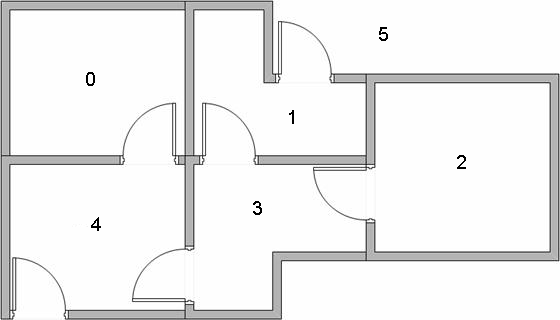
\includegraphics[width=\textwidth,height=\textheight,keepaspectratio]{1.png}
Có thể biểu diễn sơ đồ tòa nhà trên dưới dạng đồ thị có hướng như hình dưới. Mỗi đỉnh của đồ thị biểu diễn một phòng của tầng nhà (hay một trạng thái của tác tử). Nếu có cửa trực tiếp từ phòng này tới phòng kia thì ta có 1 cạnh nối giữa 2 đỉnh tương ứng (biểu diễn hành động của tác tử).\\
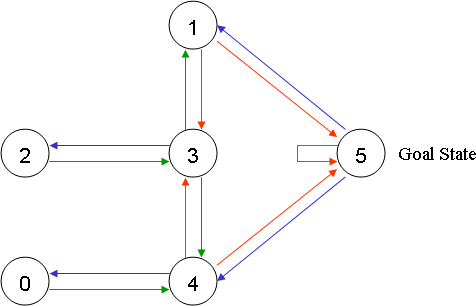
\includegraphics[width=\textwidth,height=\textheight,keepaspectratio]{2.png}
\\
Trọng số của cạnh là phần thưởng cho tác tử khi di chuyển giữa từ phòng này tới phòng kia. Do mục tiêu là thoát khỏi tầng nhà nên hành động trực tiếp thoát ra khỏi tòa nhà được thưởng cao (chẳng hạn được 100 điểm), trong khi những hành động khác không được thưởng (0 điểm) hoặc thậm chí trừ điểm (-1 điểm). Chẳng hạn từ phòng 1 có cửa trực tiếp tới phòng 5 nên cạnh nối đỉnh 1 tới đỉnh 5 có trọng số 100. Từ phòng 1 tới phòng 3 vẫn không thoát được ra ngoài nên cạnh nối từ đỉnh 1 tới đỉnh 3 có trọng số 0, từ phòng 1 không tới trực tiếp được phòng 2 nên cạnh nối từ đỉnh 1 tới đỉnh 2 có trọng số -1. Ta giả sử tác tử bắt đầu từ phòng 2 và cần đi tới phòng 5.\\
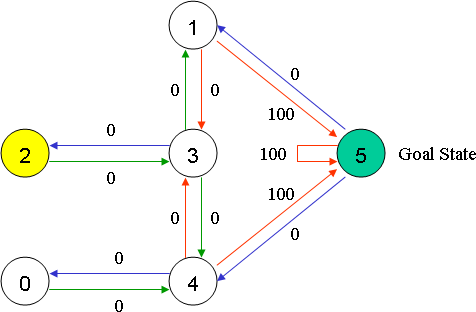
\includegraphics[width=\textwidth,height=\textheight,keepaspectratio]{3.png}
\\
	Thuật toán diễn ra như sau:
\begin{enumerate}
\item Khởi tạo $\gamma$, ma trận phần thưởng R
\item Khởi tạo Q là một ma trận 0
\item Khởi tạo trạng thái ban đầu
\item Lặp các bước sau cho tới khi đạt tới trạng thái mong muốn
\begin{itemize}
\item Chọn một hành động bất kỳ trong số tất cả các hành động có thể theo trạng thái hiện tại
\item Xác định trạng thái tiếp theo
\item Với mỗi hành động có thể, xác định giá trị Q đạt được ứng với trạng thái tiếp theo. Chọn ra hành động cho giá trị Q cao nhất
\item Tính laị giá Q theo công thức \ref{eq17}
\item Chuyển trạng thái hiện tại thành trạng thái tiếp theo vừa xác định ở trên và lặp.
\end{itemize}
\end{enumerate}
Trong ví dụ này, môi trường là tất định, hệ số học tối ưu $\alpha$ 1. Công thức của thuật toán Q-learning được rút gọn thành:
\begin{center}
$Q(x_t,a_t) = R(x_t,a_t)+\gamma max_aQ(x_{t+1},a_t)$\\
\end{center}
Ta có ma trận phần thưởng trạng thái-hành động tương ứng\\
Khởi tạo ma trận Q là ma trận 0 cỡ $6 \times 6$, hệ số chiết khấu $\gamma = 0.8$\\
$$Q=\begin{bmatrix}
0&0&0&0&0&0\\
0&0&0&0&0&0\\
0&0&0&0&0&0\\
0&0&0&0&0&0\\
0&0&0&0&0&0\\
0&0&0&0&0&0\\
\end{bmatrix}$$\\
Chọn một trạng thái bất kỳ làm trạng thái ban đầu, chẳng hạn  trạng thái 1. Có 2 trạng thái có thể đạt tới đó là trạng thái 3 và trạng thái 5. Chọn ngẫu nhiên, chẳng hạn trạng thái 5. Tính lại Q(1,5):
$$Q(1,5)=R(1,5)+0.8*\text{max}[{Q(5,1);Q(5,4);Q(5,5)}]=100+0.8*0=100$$
Ma trận Q được cập nhật lại:
$$Q=\begin{bmatrix}
0&0&0&0&0&0\\
0&0&0&0&0&100\\
0&0&0&0&0&0\\
0&0&0&0&0&0\\
0&0&0&0&0&0\\
0&0&0&0&0&0\\
\end{bmatrix}$$\\
Như vậy là đã đạt được trạng thái kết thúc. Chúng ta thử một  kịch bản khác bằng việc chọn trạng thái bắt đầu là trạng thái 3. Từ trạng thái này ta chọn một trong các trang thái có thể đạt đến: 1, 2 hoặc 4. Giả sử ta chọn 1. Khi đang ở trạng thái 1. Ta tính lại Q(3,1):
$$Q(3,1)=R(3,1)+0.8*\text{max}[{Q(1,2);Q(1,5)}]=0+0.8*100=80$$
Ma trận Q được cập nhật.
$$Q=\begin{bmatrix}
0&0&0&0&0&0\\
0&0&0&0&0&100\\
0&0&0&0&0&0\\
80&0&0&0&0&0\\
0&0&0&0&0&0\\
0&0&0&0&0&0\\
\end{bmatrix}$$\\
Từ trạng thái 1 ta có thể đến được trạng thái 3 hoặc trạng thái 5. Giả sử ngẫu nhiên ta chọn trạng thái 5. Q(1,5) được tính lại tương tự như trên. Kịch bản này lại kết thúc và ma trận Q thu được:
$$Q=\begin{bmatrix}
0&0&0&0&0&0\\
0&0&0&0&0&100\\
0&0&0&0&0&0\\
0&0&0&0&0&0\\
0&0&0&0&0&0\\
0&0&0&0&0&0\\
\end{bmatrix}$$\\
Cứ như vậy ta đề ra toàn bộ các kịch bản có thể xảy ra. Quá trình trên hội tụ dẫn đến ma trận Q cuối cùng là:
$$Q=\begin{bmatrix}
0&0&0&0&400&0\\
0&0&0&320&0&500\\
0&&0&320&0&0\\
0&400&256&0&400&0\\
320&0&0&320&0&500\\
0&400&0&0&400&500\\
\end{bmatrix}$$\\
Có thể chuẩn hóa ma trận trên bằng cách chia tất cả các phần tử cho phần tử lớn nhất của ma trận. Ta thu được:
$$Q=\begin{bmatrix}
0&0&0&0&80&0\\
0&0&0&64&0&100\\
0&&0&64&0&0\\
0&80&51&0&80&0\\
64&0&0&64&0&100\\
0&80&0&0&80&100\\
\end{bmatrix}$$\\
Từ ma trận trên ta thu được đồ thị mới:\\
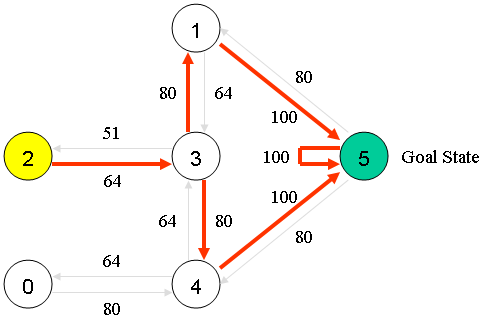
\includegraphics[width=\textwidth,height=\textheight,keepaspectratio]{5.png}
\\
Suy luận từ đồ thị, ta tìm được 1 đường đi từ trạng thái 2 tới trạng thái 5 tối ưu như sau:

\begin{enumerate}
\item Từ trạng thái 2, để Q đạt giá trị max thì di chuyển tới trạng thái 3. 
\item Từ trạng thái 3, để Q đạt max thì di chuyển tới 1 hoặc 4. Chọn di chuyển tới 1.
\item Từ trạng thái 1, để Q đạt max thì di chuyển tới 5.
\item Trạng thái 5 là trạng thái kết thúc. Thuật toán dừng. Ta thu được 1 chiến lược tối ưu: 2-3-1-5
\end{enumerate}

\chapter{Ứng dụng}
Học tăng cường có rất nhiều ứng dụng trong thực tiễn, ví dụ như áp dụng cho hệ thống điều khiển tự động các cánh tay robot công nghiêp, xe và robot tự hành, các hệ thống ứng dụng trí tuệ nhân tạo như "vua cờ vây" Alpha Go, bot game của OpenAI đã đánh bại nhiều game thủ xuất sắc trên thế giới, giải quyết bài toán "Split Delivery Vehicle Routing" trong việc quản lý chuỗi chuyển phát, thậm chí là hệ thống đánh giá các chiến lược đầu tư như Pit.AI. Còn rất nhiều các lĩnh vực khác nữa, đặc biệt là các lĩnh vực có liên quan đến trí tuệ nhân tạo đang sử dụng các phương pháp học trăng cường cho giải pháp của mình.\\
	
Trong giới hạn của báo cáo, nhóm xin trình bày một mô hình ứng dụng học tăng cường, cụ thể là thuật toán Deep Q-learning (mở rộng cho Q-learning đã trình bày ở trên) vào việc tạo ra một bot chơi game thông minh cho trò chơi Atari được mô tả như hình dưới. Trong trò chơi người chơi có nhiêm vụ điều khiển nhân vật (hình tròn đen) di chuyển (đi thẳng và rẽ theo các hướng) sao cho thu được nhiều quả táo chín (hình tròn đỏ) và tránh các quả táo độc (hình tròn xanh) trong môi trường 2D bị giới hạn. Bài toán được mô hình hóa theo phương pháp học tăng cường như sau:
\begin{itemize}
\item Tác tử là nhân vật, có khả năng đi thẳng và rẽ hướng. Để đơn giản,ta giả sử tác tử luôn luôn di chuyển, có khả năng thực hiện 5 hành động đó là rẽ theo 5 hướng khác nhau
\item Trạng thái của quá trình được thể hiện qua giá trị của các cảm biến (9 vecto). Các vecto có tác dụng thu nhận các giá trị khoảng cách của nhân vật tới vị trí của tường, táo xanh, táo đỏ.
\item Tại mỗi thời điểm, Dựa vào vị trí của tác tử trong không gian để tặng thưởng cho nó. Nếu tác tử ăn được táo đỏ (vị trí của tác tử trùng với vị trí của táo đỏ) thì nó được thưởng 1 điểm, ngược lại nếu ăn phải táo xanh thì bị trừ 1 điểm.
\item Nhiệm vụ của chúng ta là cần tìm một chiến lược điều khiển tác tử để sao cho khi kết thúc trò chơi (chẳng hạn sau 1 khoảng thời gian nào đó) điểm thưởng thu được là lớn nhất.
\end{itemize}
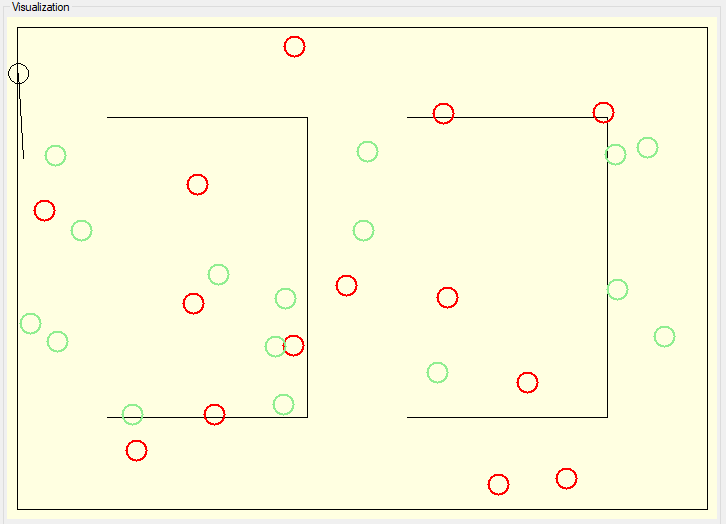
\includegraphics[width=\textwidth,height=\textheight,keepaspectratio]{6.png}
\\
Theo lý thuyết Q-learning, phần thưởng thu được của trò chơi tại thời điểm t có dạng như sau:
$$R_t = r_t+\gamma rR_{t+1}$$
Hàm $Q(x,a)$ đại diện cho phần thưởng thu được trong tương lai nếu khi thực hiện hành động a khi ở trạng thái s 
$$Q(x_t,a_t) = maxR_{t+1}$$
Hay 
$$Q(x_t,a_t) = r + \gamma max_{a'}Q(x',a')$$
Như vậy nếu như có hàm Q rồi thì việc quyết định hành động cho mỗi trạng thái trở nên đơn giản, ta chọn hành động đem lại giá trị Q lớn nhất sẽ được một chiến lược tối ưu. Có rất nhiều cách để biểu diễn hàm Q này chẳng hạn như ở dạng bảng. Trong bài toán này ta sử dụng mô hình mạng nơ ron truyền thẳng 4 lớp như sau:
\begin{itemize}
\item Lớp vào có 27 neuron
\item 2 lớp ẩn fully-connected, mỗi lớp có 50 neuron, sử dụng hàm kích hoạt là hàm relu
\item Lớp ra có 5 neuron, thê hiện giá trị tương ứng cho 5 hành động.
\end{itemize}
Hàm mất mát:
$$L=\frac{1}{2}[max_{a'}Q(x',a')-Q(x,a)]^2$$
Để huấn luyện mạng ta thực hiện như sau:
\begin{enumerate}
\item Truyền trạng thái hiện tại x qua mạng để thu được giá trị Q của tất cả các trạng thái. Tính điểm thưởng hiện tại r.
\item Thực hiện hành động theo chiến lược chọn hành động cho giá trị Q lớn nhất. Thu được trạng thái x'.
\item Truyền trạng thái x' qua mạng để thu được hành động a'. Tính lại Q-value cho hành động vừa chọn theo công thức $r+\gamma max_{a'}Q(x',a')$.
\item Thực hiện lan truyền ngược giá trị Q mới cập nhật weights.
\end{enumerate}
	Ở những vòng lặp đầu tác tử di chuyển một cách ngẫu nhiên và hoàn toàn không có khái niệm về táo xanh hay táo đỏ. Sau một thời gian huấn luyện đủ lâu, Q-loss giảm dần, và ta quan sát thấy tác tử di chuyển ngày một thông minh, tránh được những quá táo xanh, tránh được tường và cố gắng thu thập nhiều táo đỏ. Môi trường được biến đổi một cách ngẫu nhiên, chẳng hạn như vị trí xuất hiện táo xanh và táo đỏ bị thay đổi nhưng tác tử vẫn thích nghi tốt.

%============================
%Tài liệu tham khảo
\begin{thebibliography}{12}
\addcontentsline{toc}{chapter}{\quad\  \bf Tài liệu tham khảo}
\bibitem{1}Csaba Szepesvári, 2009, {\it Algorithms for Reinforcement Learning} Morgan and Claypool Publishers
\bibitem{2}David Silver, {\it Reinforcement Learning}
\bibitem{3}Richard Sutton, 2014, {\it  Reinforcement Learning: An Introduction} Kluwer Academic Publishers
\bibitem{4}{\it https://medium.com/machine-learning-for-humans/reinforcement-learning-6eacf258b265}
\bibitem{5}{\it http://simplecore-dev.intel.com/nervana/wp-content/uploads/sites/55/2015/12/ProofQlearning.pdf} 
\end{thebibliography}

\end{document}
